\documentclass{article}
\usepackage[utf8]{inputenc}

\usepackage{mathtools, amsmath, amssymb, amstext, amsfonts, mathrsfs, booktabs}
\usepackage[dvipsnames]{xcolor} % to show colorful code
\usepackage{colortbl}
\usepackage{natbib}
\usepackage[nottoc]{tocbibind} % to have the Bibliography listed as a point in the table of contents
\usepackage{setspace} % to write with 1.5 spacing
\usepackage{graphicx}
\usepackage{blkarray} % to use the blockarray
\usepackage{longtable} % to have tables span more than one page
\usepackage{tikz, xparse} %for the graphs
\usetikzlibrary{shapes, fit,positioning}
\usepackage{subcaption} % to fit two graphs next to each other
\usepackage{adjustbox} % to rotate a table
\newcommand{\comm}[1]{} % for doing comments longer than one line
\newcommand{\got}{\textit{A Game of Thrones}}
\usepackage{listings} % to display the code
\usepackage{color}
\lstset{ %
  language=R,                     % the language of the code
  basicstyle=\footnotesize,       % the size of the fonts that are used for the code
  numbers=left,                   % where to put the line-numbers
  numberstyle=\tiny\color{gray},  % the style that is used for the line-numbers
  stepnumber=1,                   % the step between two line-numbers. If it's 1, each line
                                  % will be numbered
  numbersep=5pt,                  % how far the line-numbers are from the code
  backgroundcolor=\color{white},  % choose the background color. You must add \usepackage{color}
  showspaces=false,               % show spaces adding particular underscores
  showstringspaces=false,         % underline spaces within strings
  showtabs=false,                 % show tabs within strings adding particular underscores
  frame=single,                   % adds a frame around the code
  rulecolor=\color{black},        % if not set, the frame-color may be changed on line-breaks within not-black text (e.g. commens (green here))
  tabsize=2,                      % sets default tabsize to 2 spaces
  captionpos=b,                   % sets the caption-position to bottom
  breaklines=true,                % sets automatic line breaking
  breakatwhitespace=false,        % sets if automatic breaks should only happen at whitespace
  title=\lstname,                 % show the filename of files included with \lstinputlisting;
                                  % also try caption instead of title
  keywordstyle=\color{MidnightBlue},      % keyword style
  commentstyle=\color{darkgray},   % comment style
  stringstyle=\color{PineGreen},      % string literal style
  %escapeinside={\%*}{*)},         % if you want to add a comment within your code
  morekeywords={*,...}            % if you want to add more keywords to the set
} 
\definecolor{darkgray}{gray}{0.25}
\definecolor{gray}{rgb}{0.5,0.5,0.5}
\definecolor{mauve}{rgb}{0.58,0,0.82}

%\pagestyle{headings} %to display headers, the normal way
\usepackage{fancyhdr} % to display headers, the fancy way
\pagestyle{fancy}
\fancyhf{}
\rhead{Lisa Gotzian, September 2018}
\lhead{A Game of Networks}
\rfoot{Page \thepage}

\usepackage{hyperref} % has to be the last package imported
\hypersetup{
    colorlinks=false, % the next lines only work if set to true
    linkcolor=blue,
    filecolor=magenta,      
    urlcolor=cyan,
}

\begin{document}

\begin{titlepage}
    \begin{center}
        
\includegraphics[width=0.4\textwidth]{leuphanalogo}       
        \vspace*{1cm}
        
        \huge
        \textbf{Does a social network analysis of \textit{Game of Thrones}\\ explain who will die and who will sit on the throne?}
        
        \vspace{0.5cm}
        \LARGE
        A Game of Networks \\ using \texttt{R} and \texttt{igraph}
        
        \vspace{2.5cm}
        \large
        \textbf{Lisa Gotzian}\\
        
        \vfill
        \large
        A paper presented for the course \\
        \textbf{Social Network Analysis}\\
        for the module\\
        \textbf{Reflecting Research Mehtods}\\
        instructed by\\
        \textbf{Prof. Dr. Jacqueline Loos}\\
        in the Master's Program\\
        \textbf{Management \& Data Science}
        
        \vspace{0.8cm}
        
        September 15, 2018
        
    \end{center}
\end{titlepage}
\thispagestyle{empty} % to not have a header
\tableofcontents
\newpage
\section{Introduction} \label{sec:intro}
\textit{Warning: If the reader happens to be unfamiliar with the show} Game of Thrones\textit{, he shall be warned for this paper is dark and full of spoilers.}\\

\noindent
\textit{"When you play a game of thrones you win or you die."}\\
- Cersei Lannister in \got\\
by George R. R. Martin \citep{martin1996a}\\

The iconic TV show \got{}
is characterized by its range of main characters as well as its unneglectable disposition to also have these main characters killed. Not only does the show count more than 150 characters that appear at least three times in the first books, it has more than half of these (63\%) dead by the end of season 7. Most characters' main motive is to gain power and by that to sit on the iron throne. Their willingness to become the ruler of the seven kingdoms, regardless of other people's lives, is the story told in \got.\\
This paper will examine the characters from the very first book and season as well as their relationships among each other. Will these constellations give away an estimate for who will die in season 7 or who could potentially rule the seven kingdoms? As season one mostly is based on the first book \got, the show and the book are treated equally. The few connections of the first season to the second book \textit{A Clash of Kings} \citep{martin1998a} have been neglected for this paper.\\
As \got{} is a commonly researched area for network analysis \citep{beniwal_network_2018, glander_another_2018, networkofthrones_networks_2017}, this paper contributes to the discussion by taking positive and negative relationships between the characters into account. As the show is based on a dense network of allegiances and enemies, characters with the same amount of connections might face completely opposite challenges and threats depending on the amount of support and aversion targeted towards them. Furthermore, dead characters are given special priority in this paper. If said character with numerous connections mostly faces negative attitudes towards him or her, it could be more likely for him or her to die earlier. Hence, this paper will examine this connection of relationship quality and death or power in \got.
\section{Method} \label{sec:method}
The social network presented here is based on an estimate of the many characters' connections in \got. The table follows Beniwal's approach and dataset \citep{beniwal_network_2018}, but includes positive and negative weights indicating a supportive or averse relationship. "Two characters are considered to co-occur if their names appear in the vicinity of 15 words from one another in the books" \citep{beniwal_network_2018} and characters with fewer than three interactions haven't been included either. The number of occurrences then is denoted as the weight of the tie, which is then rated by a "+" or "-". A "-" has only been used if the characters truly oppose each other, a positive attitude towards each other and a mere coexistence have been labeled as "+". Even if not all "+" relationships support each other fully, low support is also reflected in the number of occurrences. The table is structured as follows:

\begin{table}[h!]
\centering
 \begin{tabular}{llr}
 \toprule
\textbf{Source}	&	\textbf{Target}	&	\textbf{Weight}	\\
\midrule
    Alliser-Thorne	&	Jon-Snow	&	-	32	\\
    Alliser-Thorne	&	Samwell-Tarly	&	-	8	\\
    Arya-Stark	&	Cersei-Lannister	&	-	12	\\
    Arya-Stark	&	Joffrey-Baratheon	&	-	39	\\
    Arya-Stark	&	Petyr-Baelish	&	-	3	\\
    Benjen-Stark	&	Cersei-Lannister	&	-	3	\\
    Aemon-Targaryen-(Maester-Aemon)	&	Jon-Snow	&	+	34	\\
    Aemon-Targaryen-(Maester-Aemon)	&	Samwell-Tarly	&	+	5	\\
    Arya-Stark	&	Benjen-Stark	&	+	3	\\
    Arya-Stark	&	Bran-Stark	&	+	14	\\
    Arya-Stark	&	Catelyn-Stark	&	+	5	\\
    Arya-Stark	&	Eddard-Stark	&	+	30	\\
    Arya-Stark	&	Jon-Snow	&	+	37	\\
    Arya-Stark	&	Rickon-Stark	&	+	7	\\
    Arya-Stark	&	Robb-Stark	&	+	15	\\
    Arya-Stark	&	Sansa-Stark	&	+	104	\\
    ... & ... & ...\\
 \bottomrule
\end{tabular}
\caption{A part of the adjacency list with weights for the characters' connections.}
\label{table:data}
\end{table}

The network graph has been analyzed using \texttt{R} and the \texttt{igraph} package. The package offers the convenience to calculate the most important measures while also enabling complex plots.\\
The graph itself is a complete undirected one-mode network, all actors come from the same dataset.  Relations are modeled as co-occurences and attitudes. Different centrality measures will give estimates about who might be the most important character in the show. The cluster method used is a random walk cluster.

\begin{figure}
    \centering
    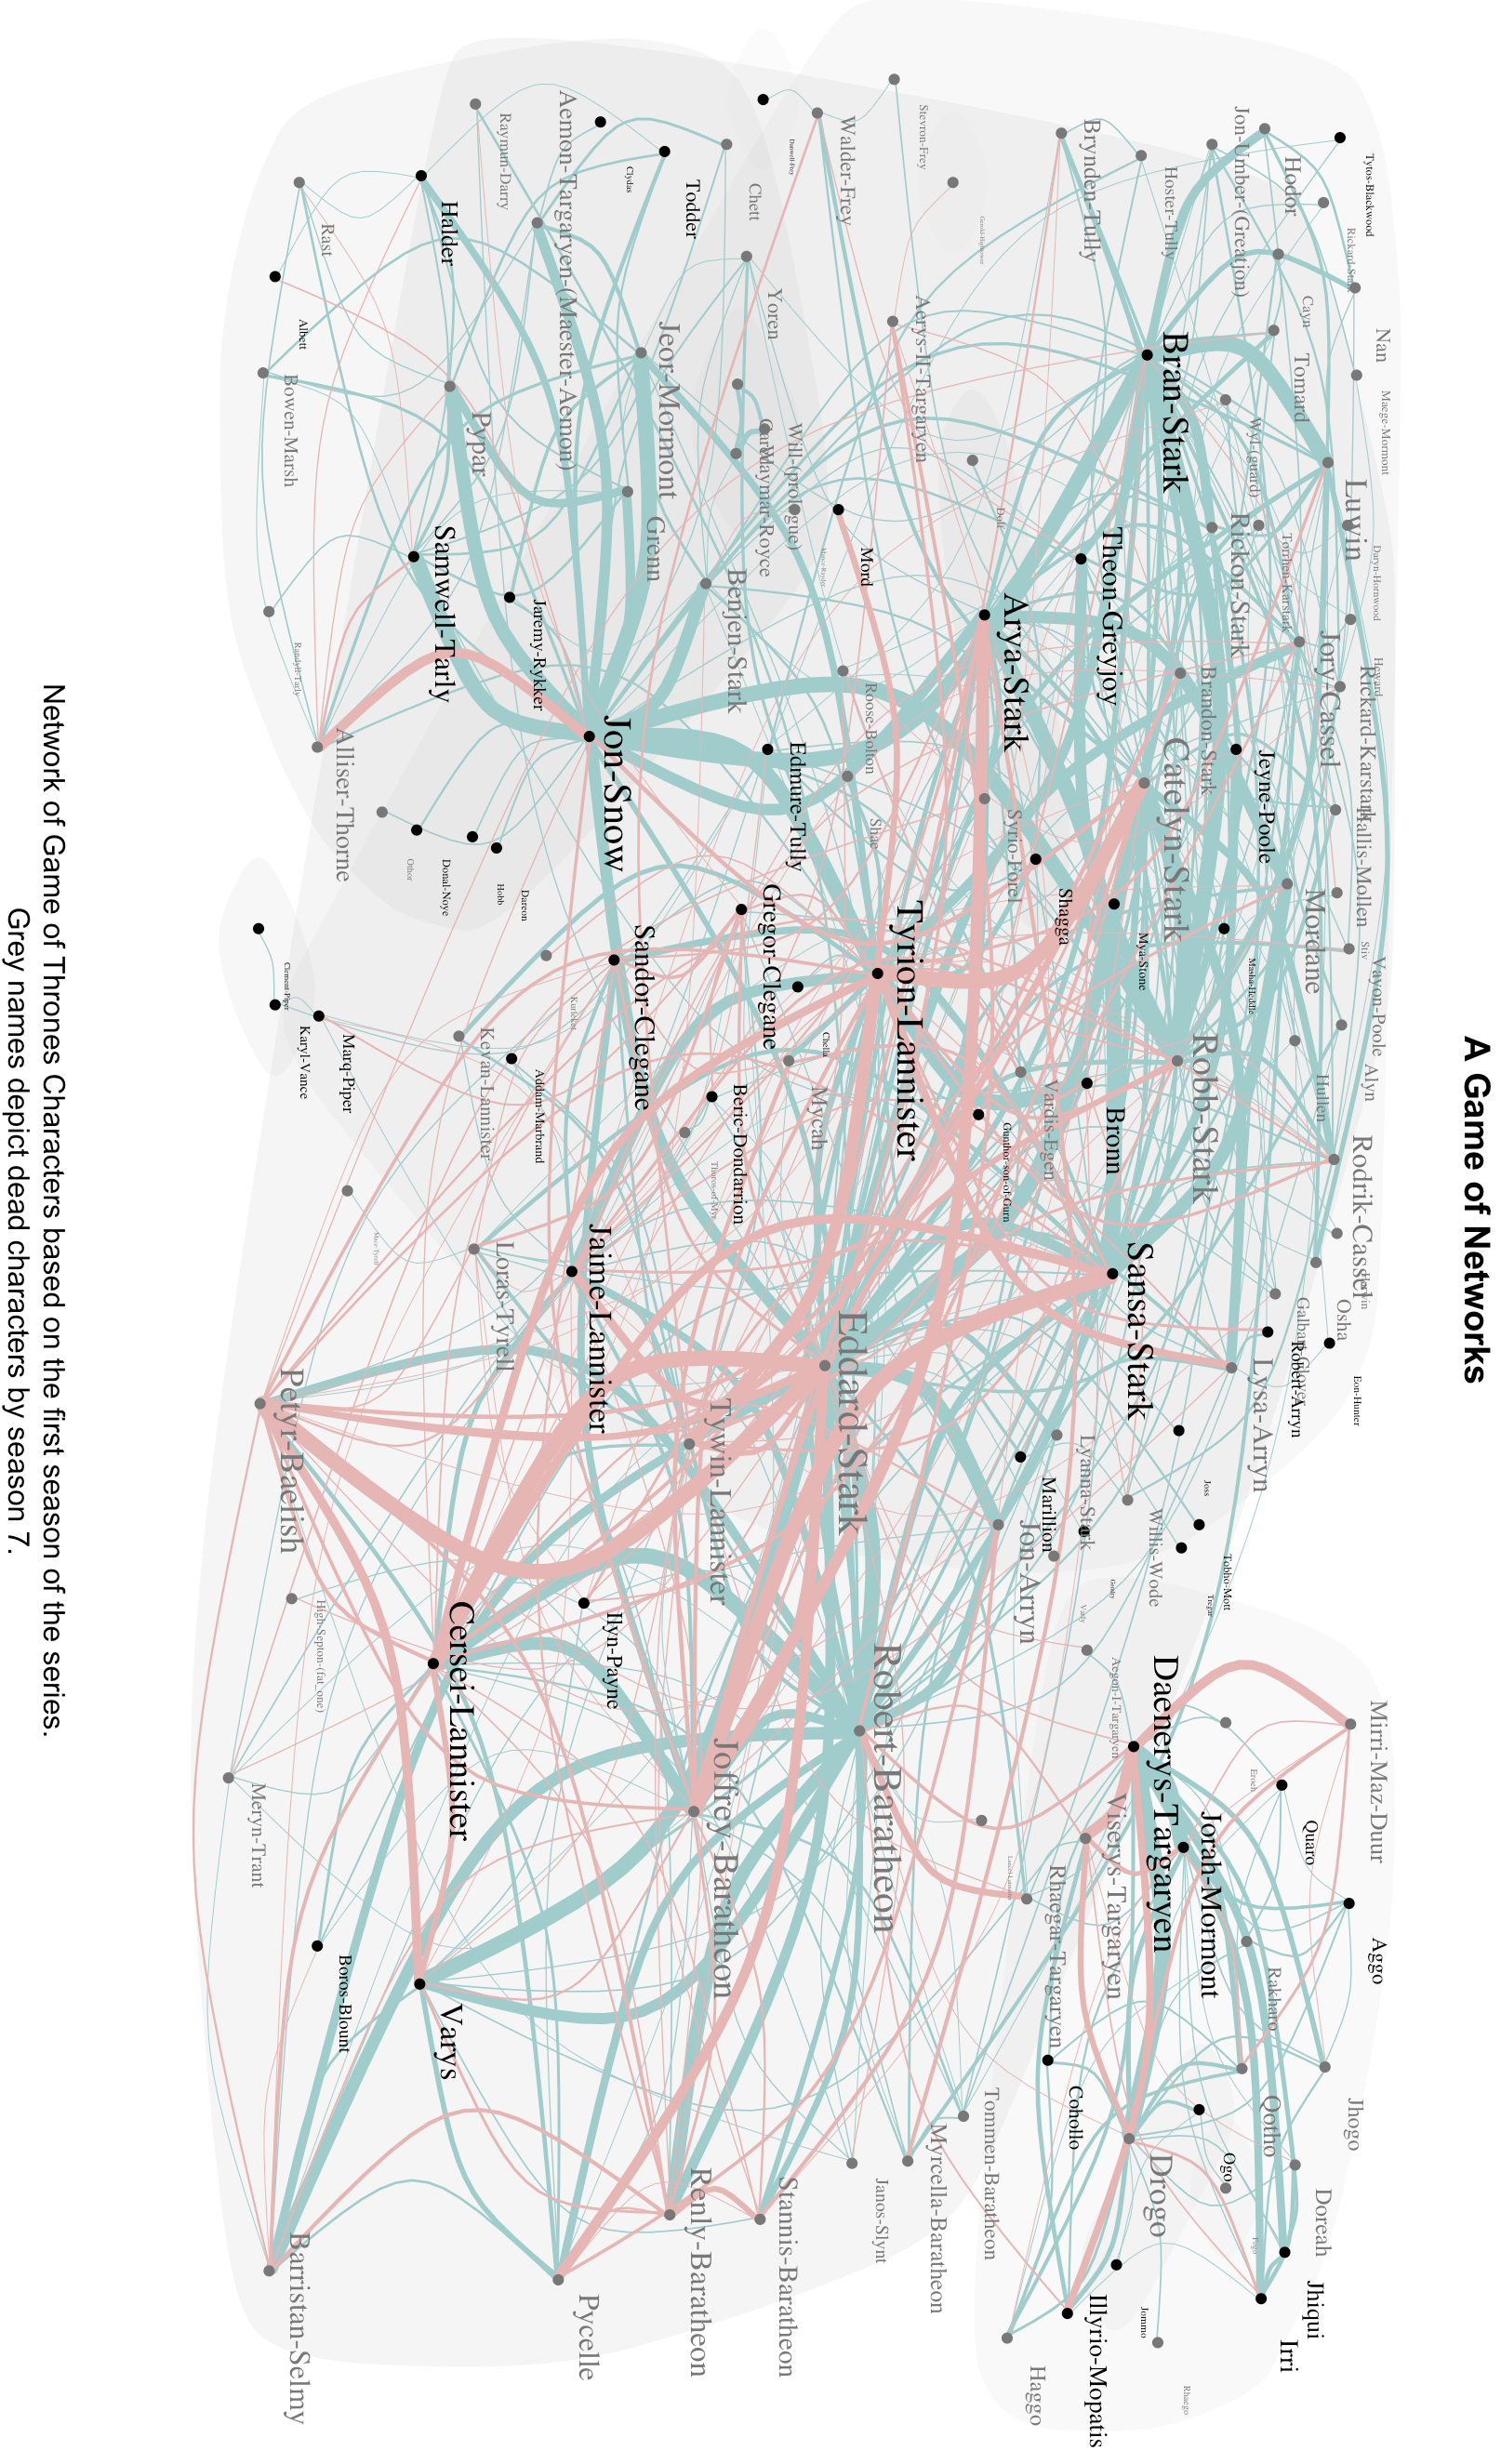
\includegraphics[scale=0.4]{plots/GOTplot.png}
    \caption{The social network of \got.}
    \label{fig:GOTplot}
\end{figure}
\section{Results} \label{sec:results}
\subsection{Overview}
Table \ref{table:data} serves as an adjacency list to create the social network of the first season of the show. For figure \ref{fig:GOTplot}, each line in the table corresponds to an undirected edge or link while each source or target becomes a node or actor. The weight is used to indicate the strength of the edge drawn, the "+" or "-" determine the color used in the graph. Additionally, all dead characters are greyed out.
The resulting plot creates a concise picture of how the positive and negative ties interplay with the actors’ power and how he or she is perceived within the network.
The full code can be found in the appendix, the code in listing \ref{lstlisting:plot} creates figure \ref{fig:GOTplot}.\\

\begin{lstlisting}[caption={Creating the plot of all characters.}, label={lstlisting:plot}] 
### Creating the final plot
plot(GOTgraph, edge.color=E(GOTgraph)$Type,# step 1: positive edges and negative edges get different colors
     vertex.color = V(GOTgraph)$Deadcolor, # step 2: dead characters become grey
     vertex.label.color = V(GOTgraph)$Deadcolor, # step 2
     edge.width = E(GOTgraph)$weightadj/3, # step 3: edges become thicker if two characters know each other better
     
     vertex.size = 1, #step 4: the nodes as such become small,...
     vertex.label.cex = log(GOTnodestrength)/5, # step 4 .... only the names become bigger based on their degree times the edge weights. The label size has been scaled by taking the natural logarithm of half the degree. This way, the small nodes don't diminish.
     vertex.label.dist = 1, # step 4, to have the labels next to the node
     
     mark.groups = GOTcluster, # step 5: mark the clusters
     mark.col = gray.colors(12, start = 0.6, alpha = 0.1), mark.border = NA, # step 5
     
     layout = GOTcoord, asp=0, #step 6,
     # with the coordinates by hand from tkplot() and without an aspect ratio
     
     ### Some layout adjustments
     vertex.frame.color = NA, # remove the frame from the vertex
     edge.curved = TRUE, # curved edges
     main = "A Game of Networks", # add a title
     sub = "Network of Game of Thrones Characters based on the first season of the series.
     Grey names depict dead characters by season 7.") 
# View this graph in the zoomed plot window and pull it to full size. The aspect ratio has been removed. 
\end{lstlisting}

\subsection{Global Measures}
The characters in \got seem to be fairly well connected. Not only does the world created by George R. R. Martin count 150 characters important enough to have shown up 3 or more times in the books or the show, it also has a large amount of edges and connections. Given the show expands over hundreds of miles which the characters walk by foot, it is remarkable that the average distance between two characters is $\langle d \rangle = 2.79$, see figure \ref{fig:plots1}. Thus when meeting a new person, every character on average knows someone that knows this new person. The people are well-connected even if it takes days to reach and visit each other. This is also displayed in the high density of 0.055.\footnote{Most networks are sparse with a much lower density \citep{RevModPhys.74.47}, a complete graph would have $L$ edges with $L=L_{max} = \binom{N}{2} = \tfrac{N(N-1)}{2} = 11,175$ in this case. This graph has 500 ties, even after the threshold of a minimum of 3 co-occurrences has been applied.}

\begin{figure}
    \centering
    \begin{subfigure}[c]{0.45\textwidth}
    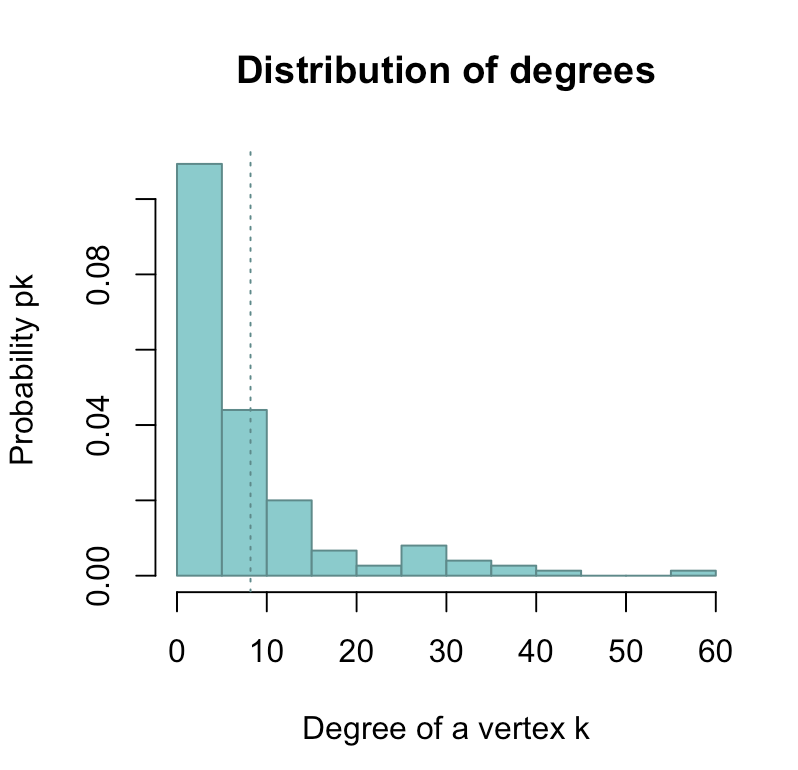
\includegraphics[scale=0.4]{plots/degreedistribution.png}
    \end{subfigure}
    \begin{subfigure}[c]{0.45\textwidth}
    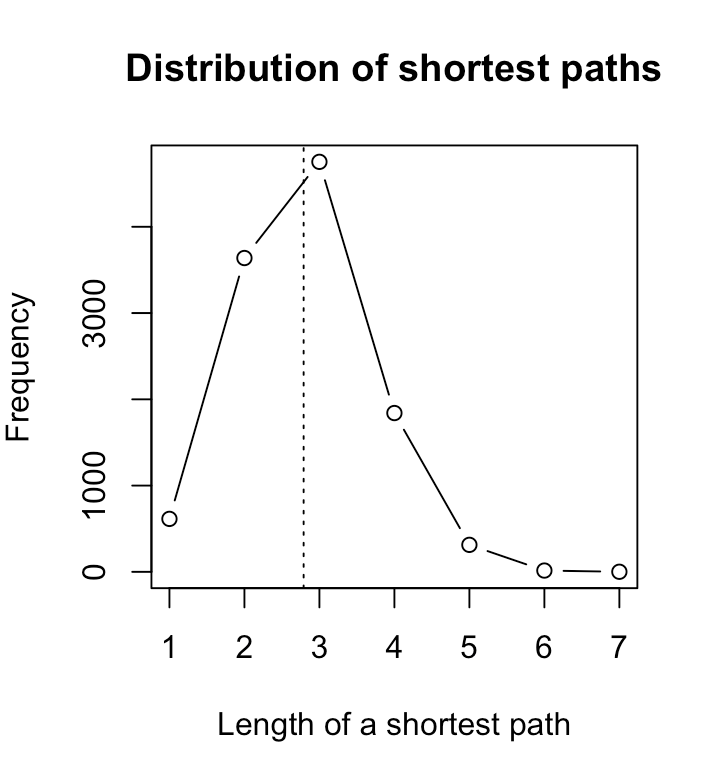
\includegraphics[scale=0.4]{plots/shortestpaths.png}
    \end{subfigure}
    \caption{Distributions of degrees and shortest paths of the network.}
    \label{fig:plots1}
\end{figure}

On average, each characters knows $\langle k \rangle = 8.187$ other characters, though most characters know 5 or less people, see figure \ref{fig:plots1}. The distribution of degrees $p_k$ follows a power law distribution,\footnote{$\alpha = 2.170$, the Kolmogorov-Smirnov test couldn't reject a power law distribution.} as it is common among sparse networks \citep{RevModPhys.74.47}. This means that the network includes a number of hubs, very central vertices that connect other nodes. Given that this is a classical fictional story that has to have some focus on a set of characters, the occurrence of hubs or main characters isn't too surprising. 

\begin{table}[h]
    \centering
    \begin{tabular}{lcr}
    \toprule
    \textbf{Measure} & & \\
    \midrule
    Order (Number of vertices) & $|V| = n$	&	150 \\
    Size (Number of edges) & $|E| = m$	&	614 \\
    Density for undirected networks & $\tfrac{2m}{n(n-1)}$	&	0,055\\
    Clustering coefficient/Transitivity & &	0,365\\
    Diameter of $G$ (length of longest shortest path) & &	48\\
    Average distance & $\langle d \rangle$ &	2,79\\
    Average degree & $\langle k \rangle$ & 8.187\\
    \bottomrule
    \end{tabular}
    \caption{Global measures of the network.}
    \label{tab:globalmeasures}
\end{table}

\newpage
\subsection{Local Measures}
Let's take a closer look at the characters itself and especially the most central and the best-connected people. Given the network in figure \ref{fig:GOTplot}, there are some very firm candidates for being a hub in \got. Most of the central characters are  from the Lannister and Stark family - like Tyrion Lannister, Eddard Stark, Sansa Stark or Robb Stark, all of them listed in high positions in table \ref{table:comparison} that compares the centrality of the characters. Family ties and a supportive network are a tremendous gift in times of trouble like present in \got, and the two big families own the support by birth.\\
On the other hand, Daenerys Targaryen and Jon Snow seem to be bridges for two communities outside of the main plot. The grey areas determine the subgroups found by \texttt{cluster\_walktrap()} which correspond quite well to the two communities Daenerys and Jon live in. When Jon joined the very remote \textit{Night's Watch} to protect the realm from anything north of the wall, he gained a network among the guards at the wall. Coming from the House of Stark, he nevertheless has strong connections to his family as well. He even ranks third among the strength of positive connections, see table \ref{table:comparison}. Daenerys, the former mad king's daughter, lives rather isolated with the folk of the \textit{Dothraki}. By being far away from King's Landing and the present king, she doesn't run the risk of being killed by the intrigues around the throne. Both Jon and Daenerys survived till season 7, surviving Robert Baratheon,\footnote{Robert had quite a positive network. It should be mentioned that Robert died while hunting and being drunk.} his elder son Joffrey Baratheon and his younger son Tommen Baratheon as kings, not to mention the numerous claims to the throne such as by Stannis Baratheon and Renley Baratheon. An explanation of the failed claims could be the lack of overwhelming support other characters rely on, as both are not well connected. In the most recent season, Jon and Daenerys met and fell in love while both of them have built their network further, gaining more and more support. The isolation of both in the first season seems to be a strong indicator for later success. A wide range of fans currently suspects the two to sit on the Iron Throne in the end \citep{ziss_9_2018}.\\
A tragic character of the very first season is Eddard Stark. According to degree, strength and eigencentrality, he is the most central character, ranking 2 in betweenness as well, see figure \ref{table:comparison}. When the old hand of the king\footnote{The advisor to the king and the most important person in the realm besides the king himself.} died, Robert Baratheon, the king, turned to his old friend Ned for help. Ned couldn't possibly neglect the offer, so the honorable Lord Stark made his way to King's Landing. Soon enough, his honesty endangered powerful intrigues to be disclosed, resulting in a devastating loss of support for him. Quite a few people wished to see Ned Stark dead, his \textit{StrengthMinus} value with only the negative relationships is higher than any other character's. Ned Stark seems to have gotten too deep into the network of Thrones while he righteously intended to reveal a number of dark secrets. This probably is the reason for him being killed after all in the middle of a very aversive network around him. Unfortunately for House Stark, the Lannisters make sure to not only kill Ned Stark but also his many supporters and guards, indicated by the many grey names among the Stark family in figure \ref{fig:GOTplot}.\\
His fate is in a way comparable to Joffrey Baratheon's, Petyr Baelish's and Tywin Lannister's fate. Though in contrast to Lord Stark, all of the three more or less openly met other characters with distrust, hate and aversion, they managed to build a very negative network as well. Hence, one of their opponents seems to have been witty or strong enough to murder them. This also means that social ties are connected: if the heir of House Stark, Sansa Stark in this case, is against Petyr Baelish, she will turn other people’s attitudes  towards him as well. All four characters impressively show the importance of a supportive network, especially when one ranks high in centrality of the network and becomes the focus of attention.\\
Varys, a character known for his connections similar to Petyr Baelish, mostly uses his influence from the background. His network expands among the unknown characters who deliver the most recent and important bits of information to him. It is that unimportant that he is not even present in table \ref{table:comparison}. In contrast to Petyr Baelish, he manages to mostly employ positive relationships with the important people and by that ensures his survival in \got.\\
Among the most central nodes, an important name to mention is Tyrion Lannister. Born into a family of intrigues, he uses his wits to survive the never-ending game of survival. During the course of the seasons, he doesn't only become hand of the king twice, he also keeps a dense network of supporters and allies. Given his dwarfism, his family isn't too fond of him, but tolerates him to a certain degree.\\
When drawn together, the living actors give an interesting picture: At the end of season 7, the main forces are the side of King's Landing with Cersei and her guards as well as Daenerys and Jon. Currently, Varys, Tyrion and quite a few other characters have sided with Daenerys. With Jon involved, it could even be possible to have the Stark family on their side. Jon on the other hand will inherit major parts of his father Ned Stark's network as he is the oldest surviving son. This leads to an overwhelmingly strong opponent to the queen Cersei. If there was an ending to the show with a king or queen involved, already the network of the very first season gives away a good estimate: Daenerys and Jon.\\
Being alive and becoming king are densely interconnected. Once a certain amount of power has emerged, one would have to make sure to survive by keeping up positive relationships. Then, one has high chances to sit on the iron throne.\\
Lastly, if the show actually had a very low number of main characters like other books or shows, the graph in figure \ref{fig:measurecomparison} might look less scattered as these nodes would then be clearly denoted as central. It shows how the different centrality measures don't agree on the same nodes. Eddard Stark in dark blue and the king Robert Baratheon in blue are overall very central, the \textit{StrengthRatio} however denotes Bran Stark, Jon Snow and Robb Stark with an impressively positive network as well. Bran Stark has emerged to a very important role in season 7 while Robb fought long and hard for becoming King in the North. Robb's downfall was also due to an intrigue, Bran is still alive. Clearly, the \textit{StrengthRatio} enforces the importance of taking positive and negative edges into consideration. Despite some actors like Eddard Stark being very central, other nodes have a much higher \textit{StrengthRatio} resulting in the peak in figure \ref{fig:measurecomparison}. This is how especially Eddard Stark might have been too central in the network which lead to him being killed.

\begin{figure}
    \centering
    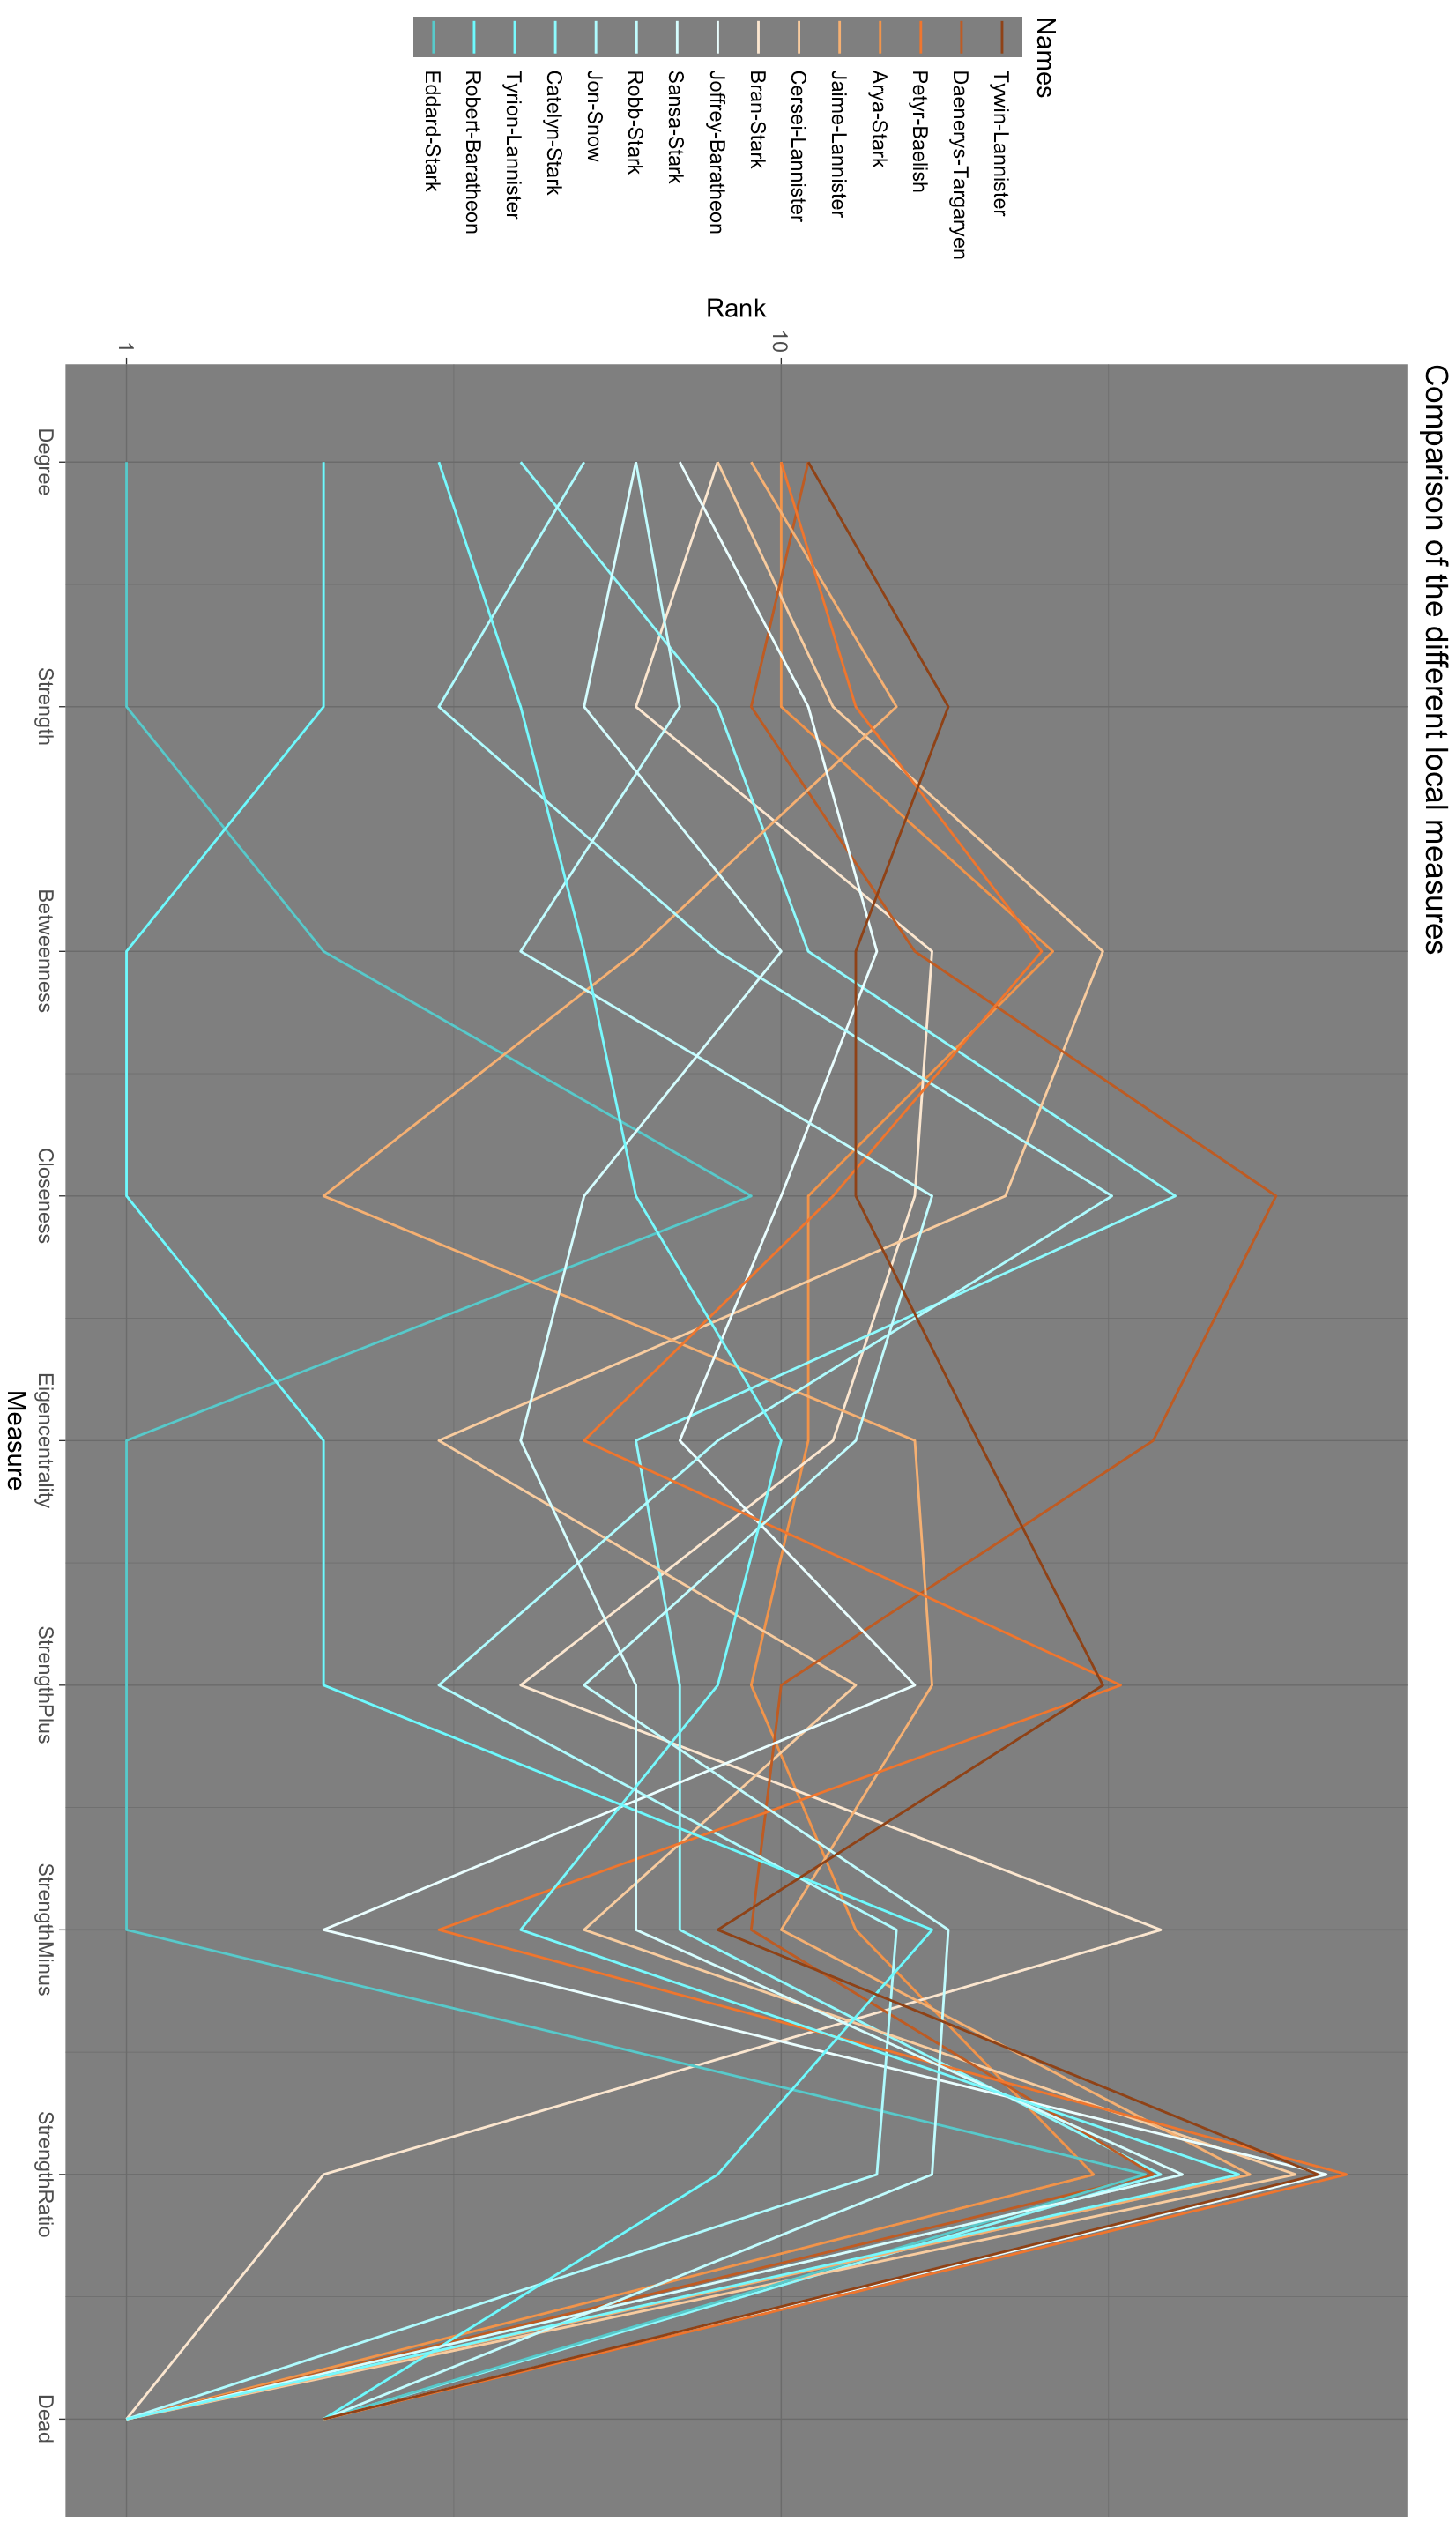
\includegraphics[scale=0.34]{plots/measurecomparison.png}
    \caption{The 15 characters with the highest degree are ranked across different local measures that somewhat represent influence and connectedness. For a better overview, a logarithmic scale was chosen. \textit{StrengthPlus} and \textit{StrengthMinus} only take the positive or negative relationships into account, hence \textit{StrengthRatio} is the ratio of the two. As the bottom of the graph usually represents a better ranking, alive characters correspond to 1, dead characters to 2 on the \textit{Dead} scale.}
    \label{fig:measurecomparison}
\end{figure}


\begin{table}
\caption{Centrality comparison of the 15 characters with the highest degree, corresponding to figure \ref{fig:measurecomparison}. The table gives away the ranks of the characters in a certain centrality measure.}
    \label{table:comparison}
    \begin{adjustbox}{angle=270}
    \begin{tabular}
    {p{2.5cm}p{0.9cm}p{1.2cm}p{1.2cm}p{0.9cm}p{1.2cm}p{1.2cm}p{1.2cm}p{1.2cm}p{0.9cm}}
    \toprule
    Names & Degree & Strength & Between-ness & Close-ness & Eigen-centrality & Strength Plus & Strength Minus & Strength Ratio & Dead\\
    \midrule
    Eddard-Stark & 1 & 1 & 2 & 9 & 1 & 1 & 1 & 36 & 0\\
    Robert-Baratheon & 2 & 2 & 1 & 1 & 2 & 2 & 17 & 8 & 0\\
    Tyrion-Lannister & 3 & 4 & 5 & 6 & 10 & 8 & 4 & 50 & 1\\
    Catelyn-Stark & 4 & 8 & 11 & 40 & 6 & 7 & 7 & 38 & 0\\
    Jon-Snow & 5 & 3 & 8 & 32 & 8 & 3 & 15 & 14 & 1\\
    \addlinespace
    Robb-Stark & 6 & 7 & 4 & 17 & 13 & 5 & 18 & 17 & 0\\
    Sansa-Stark & 6 & 5 & 10 & 5 & 4 & 6 & 6 & 41 & 1\\
    Joffrey-Baratheon & 7 & 11 & 14 & 10 & 7 & 16 & 2 & 68 & 0\\
    Bran-Stark & 8 & 6 & 17 & 16 & 12 & 4 & 38 & 2 & 1\\
    Cersei-Lannister & 8 & 12 & 31 & 22 & 3 & 13 & 5 & 61 & 1\\
    \addlinespace
    Jaime-Lannister & 9 & 15 & 6 & 2 & 16 & 17 & 10 & 52 & 1\\
    Arya-Stark & 10 & 10 & 26 & 11 & 11 & 9 & 13 & 30 & 1\\
    Petyr-Baelish & 10 & 13 & 25 & 12 & 5 & 33 & 3 & 73 & 0\\
    Daenerys-Targaryen & 11 & 9 & 16 & 57 & 37 & 10 & 9 & 37 & 1\\
    Tywin-Lannister & 11 & 18 & 13 & 13 & 20 & 31 & 8 & 66 & 0\\
    \bottomrule
    \end{tabular}
    \end{adjustbox}
\end{table}
 % this inserts the big plot and the table
\section{Discussion}
Taking the quality of a relationship into consideration lead to an improved model to explain death and the emergence of a king in \got. While the number of connections explain a big part, the support or aversion network is worth to be considered as well. The overall network seems to explain the development of the show's characters fairly well and also allows for an outlook to who might become king or queen in the new season.\\
The result of such a network however is always quite subjective, beginning with the reliability (and thus validity) due to my own rating of the social ties. Another very subjective step was the arrangement of nodes in \texttt{igraph} with \texttt{tkplot()}, the interactive graphing feature of the package. Knowing the characters made the arrangement much easier. The interpretation of this network might have then lead to the classy hindsight bias \citep{TVERSKY1973207}, in which one easily explains previous events because one knows the end of the story. The knowledge of who died definitely facilitated the analysis of how and why connections might have lead to a character's death. The estimate of a future king or queen is the only scientific statement that can be proven false in the future season 8.

\comm{Main content:
- Are the estimates by the authors realistic?
- reliability: would we be able to replicate the model with newer data? Would the construction of the model still work or is it a one-time-only model that only works with the data from 2009?
- what to enhance in the paper?
- convergence of the model? what do the plots say?}


\begin{figure}
    \centering
    
\includegraphics[scale=0.2]{tyrion.jpeg}
    \caption{Tyrion Lannister, one of the most central nodes according to a number of centrality measures, is often quoted when referring to his enormous knowledge and sociability. He is a good example for how connections and knowledge lead to power and influence.}
    \label{fig:tyrion}
\end{figure}

\bibliographystyle{apalike}
\bibliography{references}

\end{document}
